\chapter{Ground truth}
\chaptermark{Ground truth}
\label{app:groundtruth}
\graphicspath{{./chapters/Appendix/figs/}}

This appendix details the ground truth construction process, the visual (regions) and semantic information annotation, the file structure, the annotation quality assessment and finally the terms of use.
This work is the result of an close collaboration with Cl{\'e}ment Gu{\'e}rin~\cite{phdthesisGuerin14} and many meetings with the eBDtheque project team of the L3i lab.

% section term_of_use (end)

\section{Ground truth construction} % (fold)
\label{sec:ground_truth_construction}

The ground truth has been defined in accordance to existing formalism in order to fulfil the needs of a large amount of researchers related to comics material.
It integrates low and high level information such as spatial position of the elements in the image, their semantic links and also bibliographic information.


The comics art is extremely heterogeneous and our dataset voluntarily integrates albums that can be classified as
unconventional.
This leaves room for interpretation on the form which increase annotation variations by different people and decrease the uniformity of the ground truth.
This precision level is used in several, widely used datasets~\cite{pascal-voc-2012, yao2007introduction}.
%{\color{blue}This groundtruthing level is also used for well known dataset widely used~\cite{pascal-voc-2012, yao2007introduction}.}

In order to cover a wide range of possible research matters, it has been decided to extract three different types of objects from the corpus: text lines, balloons and panels.
We decided to do this first ground truth by drawing horizontal bounding boxes as close as possible from the image content and including all its pixels.
% in order to proceed a maximum of pages in the allowed time. 
We chose this level of granularity in order to limit the subjectiveness of the person making the annotation.

Hereafter we detail the two levels of annotation (visual and semantic) that form the ground truth and how they are indexed in a file.
The combination of visual and semantic annotation provides the advantage of making this ground truth relevant for document analysis and semantic evaluation which are both part of the comics understanding process.

% each element to annotate and the protocol to follow.
% follows specific guidelines according to the rules below:

\subsection{Visual annotation} % (fold)
\label{sub:visual_annotation}
The first annotation consists in defining the spatial region where elements are located in the image.
We describe here how the visual annotations have been performed for the panels, balloons, texts and comic characters.

% section visual_annotation (end)
\paragraph{Panels} % (fold)
\label{par:panels}
The frame or panels are defined as an image area, generally rectangular, representing a single scene in the story. 
There is always at least one panel per page; the entire page region can be used as panel if necessary.
When a panel has a black border, the bounding box is placed as close as possible to its frame.
Sometimes, images have not been scanned perfectly horizontally, it is then impossible to have an horizontal bounding box sticking exactly to the border.
When the panel border is partially absent or suggested by the neighbourhood, the bounding box just defines the content of the panel.
In all cases, the other elements (balloon, text, drawings) extending from the frame are truncated (Figure~\ref{fig:gt:segPanel}).

%%%%%%%%%%%%%%%%%%%%%%%%%%%%%%%%%%%%%%%%%%%%%%%%%%%%%%%%%
\begin{figure}[h!]
\begin{center}
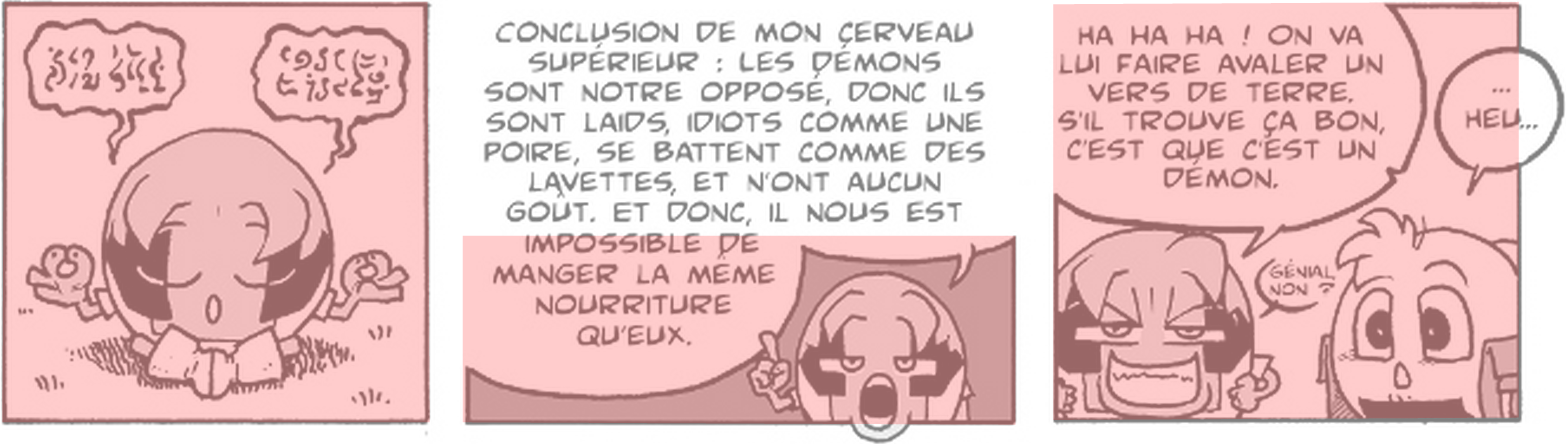
\includegraphics[width=0.8\textwidth]{segPanel.png}
\caption[Panel annotation]{Example of three panel annotations. The bounding box (transparent red) is defined without taking into account of non-panel elements in all cases.}
\label{fig:gt:segPanel}
\end{center}
\end{figure}
%%%%%%%%%%%%%%%%%%%%%%%%%%%%%%%%%%%%%%%%%%%%%%%%%%%%%%%%%

%They can be frame-less, in that case the bounding box will be set according to the contained drawings, see Fig. \ref{fig:segmentation}c. %, ignoring text and overlapping features.
%In both cases, text and overlapping features are ignored.
%There is necessarily at least one panel in a page. 
% paragraph panels (end)

% The panel reading order is also annotated in a metadata called \texttt{rank}, it is in integer  between $1$ and $n$ which is increased incrementally from the first to the last panel $n$ in an image.%, le premier de la séquence prenant la valeur $1$ et le dernier la valeur $n$ pour une page contenant $n$ cases.

\paragraph{Balloons} % (fold)
\label{par:balloons}
We define a balloon (phylactery or bubble) as the region of an image including one or several lines of text, graphically defined by an identifiable physical boundary or suggested by the presence of an arrow pointing to the speaker (the tail).
Although rare, empty balloons (not containing lines of text) are also annotated if they are clearly identifiable by their shape or
the tail representation.
Pixel level annotation follows the contour of the balloon (Figure~\ref{fig:gt:segBalloons}c), while bounding box annotation does not consider the contour of phylactery and truncates the tail.
Sometimes it crosses the entire panel and generates an unrepresentative position of the desired balloon (Figure~\ref{fig:gt:segBalloons}a).
When the balloon is not closed (e.g. open contour) the annotated contour has to stick as close as possible to the contained text (Figure~\ref{fig:gt:segBalloons}b).
Note that the first version of the ground truth (2013) has been defined at bounding box level ignoring the tail and the second version (2014) at pixel level following the contour variations and the tail region.

%%%%%%%%%%%%%%%%%%%%%%%%%%%%%%%%%%%%%%%%%%%%%%ù
\begin{figure}[h!]
\begin{center}
\begin{tabular}{ccc}
a) 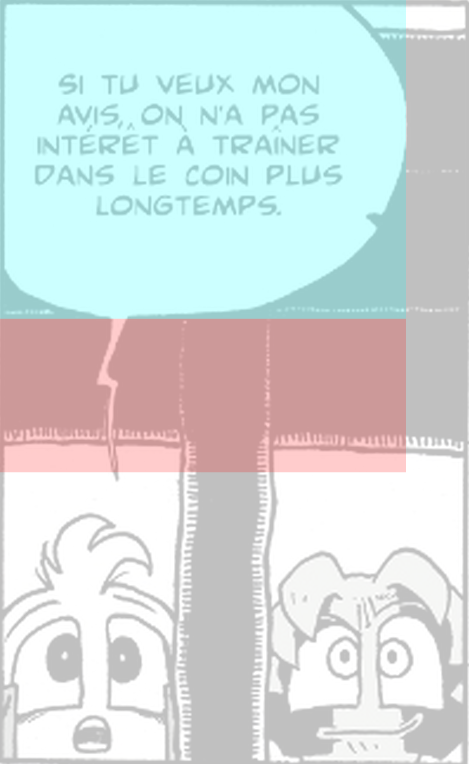
\includegraphics[width=80px]{segBalloon1.png} 
& 
b) 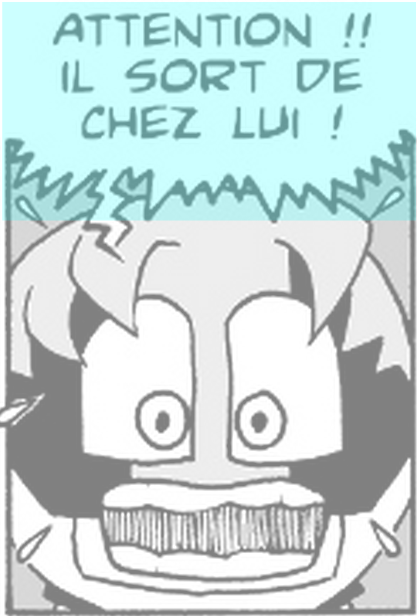
\includegraphics[width=80px]{segBalloon2.png}
&
c) 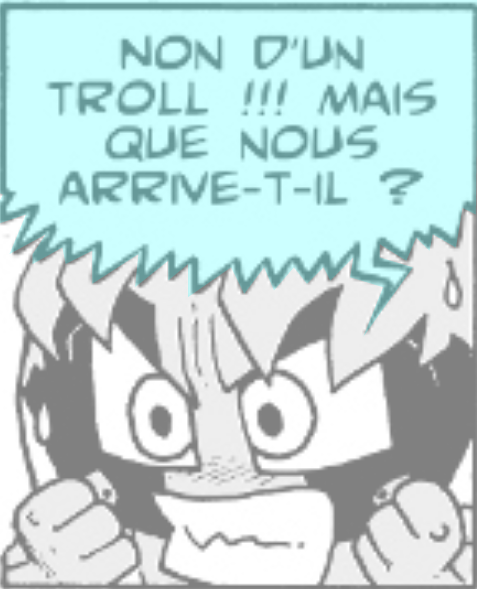
\includegraphics[width=80px]{segBalloon3.png}
\end{tabular}
\caption[Speech balloon contour annotation]{Example of balloon clipping: a) using bounding box excluding the tail, b) bounding box of non-closed balloon, c) pixel level contour annotation.} 
\label{fig:gt:segBalloons}
\end{center}
\end{figure}
%%%%%%%%%%%%%%%%%%%%%%%%%%%%%%%%%%%%%%%%%%%%%%ù

% paragraph balloons (end)

\paragraph{Text lines} % (fold)
\label{par:text_lines}
The text lines are defined as a sequence of text characters aligned in the same direction (Figure~\ref{fig:gt:segLines}a).
This definition encompasses both speech text and narrative text, often located inside balloon, onomatopoeia (graphic sound) that are written or drawn directly in the panel without particular container.
%The text of the latter, although they are occasionally parallel to the edges of the box is still clipped by a horizontal bounding box for consistency across the ground truth.
Comics are static graphics, the expression of emotions of a comic character is the joint action of drawing and text, sometimes in the form of a single punctuation symbol.
For instance, an exclamation mark for surprise or a question mark for a misunderstanding.
These isolated symbols convey information and are segmented as text line as well (Figure~\ref{fig:gt:segLines}b).
Similarly, we have chosen to include in this category the illustrative text, such as a road sign or storefront (Figure~\ref{fig:gt:segLines}c).
Although at the boundary between text and graphic, these elements are still invariably read by the reader and their annotation is potentially interesting for multiple purposes, including story and scene analysis.

%%%%%%%%%%%%%%%%%%%%%%%%%%%%%%%%%%%%%%%%%%%%%%ù
\begin{figure}[h!]
\begin{center}
\subfloat[Speech text into speech balloon]{\label{fig:ex:segLine1}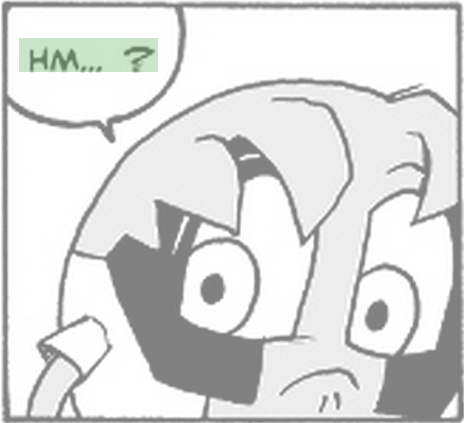
\includegraphics[width=0.3\textwidth]{segLine1.png}} \hspace{0.5em}
\subfloat[Unique symbol (punctuation)]{\label{fig:ex:segLine2}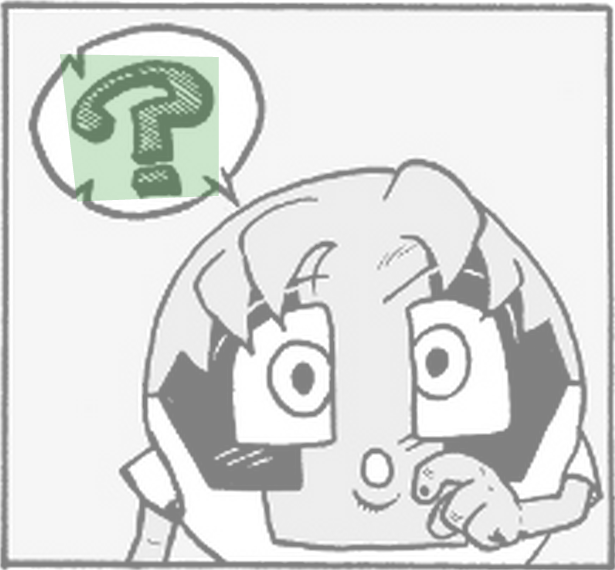
\includegraphics[width=0.3\textwidth]{segLine2.png}} \hspace{0.5em}
\subfloat[Illustrative text (non-horizontal)]{\label{fig:ex:segLine3}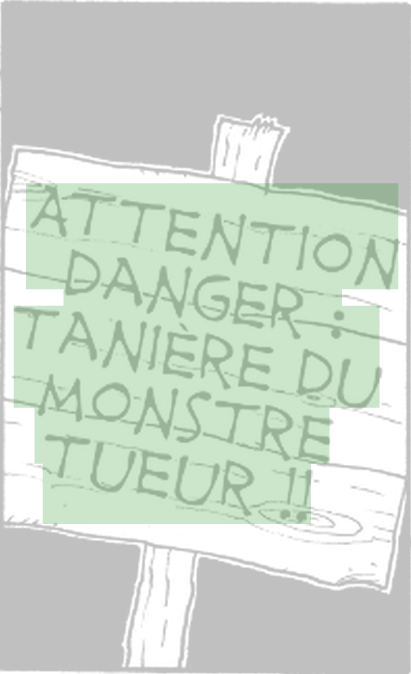
\includegraphics[width=0.3\textwidth]{segLine3.png}}

% \begin{tabular}{ccc}
% a) 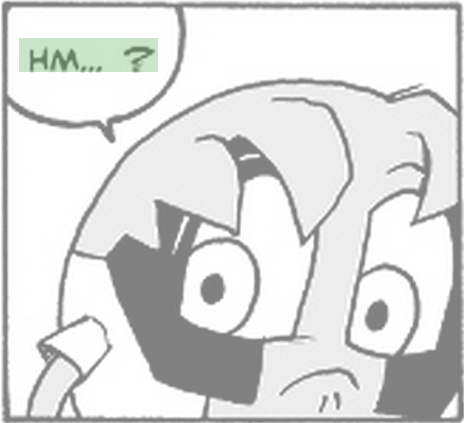
\includegraphics[width=80px]{segLine1.png} 
% & 
% b) 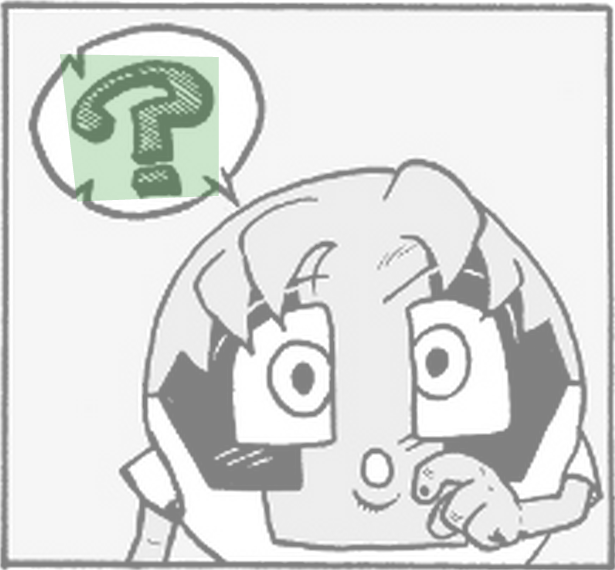
\includegraphics[width=80px]{segLine2.png}
% &
% c) 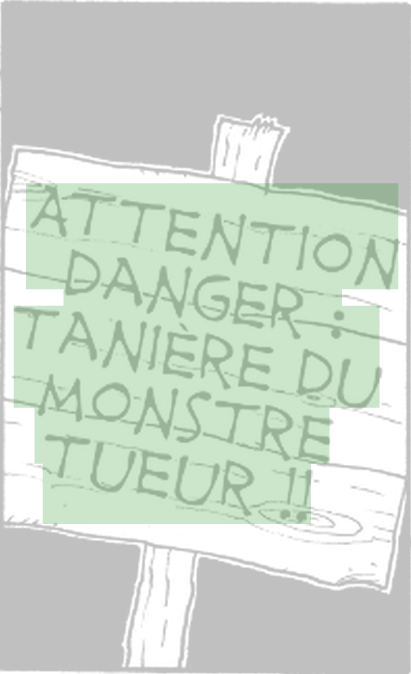
\includegraphics[width=80px]{segLine3.png}
% \end{tabular}
\caption[Position annotation of text lines]{Examples of text line position annotations.} 
\label{fig:gt:segLines}
\end{center}
\end{figure}
%%%%%%%%%%%%%%%%%%%%%%%%%%%%%%%%%%%%%%%%%%%%%%ù

% paragraph text_lines (end)

\paragraph{Comic characters} % (fold)
\label{par:comic_characters}
The comic character positions have been included in the second version of the ground truth only (2014).
The concept of ``character'' may have different interpretations when used for comics and must be specified.
Characters in a comic have not necessarily a human-like, or even living being appearance.
Even so, it would be appropriate to annotate every character instance appearing in a box while some are only part of the scenery.
Therefore, we have chosen to limit the annotation to the comic characters that emits at least one speech balloon in the album (minimal impact in the story).
Their bounding box has been defined to maximize the region occupied by the comic character inside the box region.
Therefore, some parts of the character such as arms or legs, are clipped sometimes (Figure~\ref{fig:gt:segCharacter}).

%%%%%%%%%%%%%%%%%%%%%%%%%%%%%%%%%%%%%%%%%%%%%%
\begin{figure}[h!]
\begin{center}
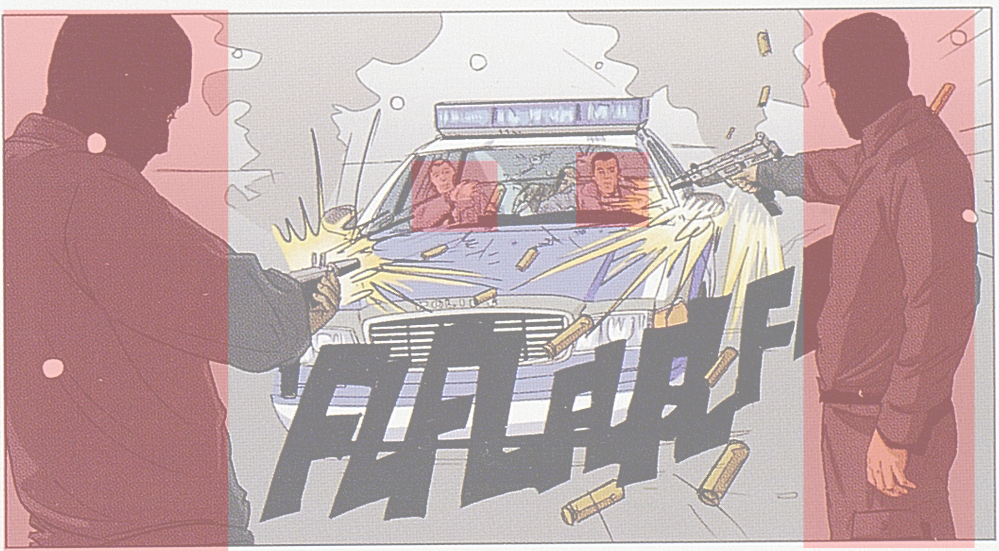
\includegraphics[width=0.75\textwidth]{segCharacter.png}
\caption[Comic character position annotation]{Example of comic character annotation: sniper's arms are not included in the bounding box in order to maximize the region occupied by the sniper in its bounding box. The two snipers and the two characters in the car are annotated because they emit a speech balloon in a different panel. Image credits:~\cite{Boston10}.}
\label{fig:gt:segCharacter}
\end{center}
\end{figure}
%%%%%%%%%%%%%%%%%%%%%%%%%%%%%%%%%%%%%%%%%%%%%%

% paragraph comic_characters (end)


% section ground_truth_construction (end)

\subsection{Semantic annotation} % (fold)
\label{sub:gt:semantic_annotation}
This second level of annotation completes each spatial region with additional information about its semantic.
Also, the image itself is annotated with extra information about its origin (e.g. album, collection, author and publisher).
%Once segmented, each object is annotated with a set of predefined metadata as follows. 

\paragraph{Images}
The images, often assimilated as pages, has been annotated with bibliographical information, so that anyone using this ground truth is free to get his own paper copy of the comic books for extra uses.
The first annotation is the page number (\texttt{{pageNumber}}) then the comic book title, from which the page has been picked up, and its release date (\texttt{{albumTitle, releaseDate}}), the series it belongs to (\texttt{{collectionTitle}}), the authors and editor names (\texttt{{writerName, drawerName, editorName}}) and, finally, the website and/or ISBN (\texttt{{website, ISBN}}).
The album title is not mandatory for webcomics.
Structural information about the page content has been added as well, such as resolution (\texttt{{resolution}}), reading direction (\texttt{{readingDirection}}), main language of the text (\texttt{{language}}) and single or double page information (\texttt{{doublePage}}).
% These annotation are stored in a tag named \texttt{{Pages}}.

\paragraph{Panels} 
The panels are annotated with a \texttt{{rank}} metadata which stands for its position in the reading sequence.
The first panel to be read on a given page has its rank property set to 1, while the last one is set to \textit{n}, where \textit{n} is the number of panels in the page.

\paragraph{Balloons}
Balloons are also annotated with a \texttt{{rank}} property that defines their reading order relatively to the image because balloons are not always included in panels.
%, their rank is set according to the page as a whole. 
For a page containing $m$ balloons, the first balloon's rank will be 1 and the last will be $m$.
%Moreover, two additional metadata are given. 
A second information concerns the \texttt{{shape}} of the balloon.
This feature conveys information about how the contained text is spoken (tone).
The type of \texttt{{shape}} is given from the following list \{\texttt{smooth, wavy, spiky, suggested, other}\} as pictured in Figure~\ref{fig:gt:balloonShape}.
Finally, the tail tip position (extremity) and its pointing direction have been added into the second version of the ground truth.
There are given through the \texttt{{tailTip}} and \texttt{{tailDirection}} properties.
The possible values of the direction are reduced to the eight cardinal directions plus a ninth additional value for the lack of tail: \{\texttt{N, NE, E, SE, S, SW, W, NW, none}\}.
In the second version of the ground truth (2014), we added the identifier of the comic character which is emitting the balloon \texttt{{idCharacter}}. 

%%%%%%%%%%%%%%%%%%%%%%%%%%%%%%%%%%%%%%%%%%%%%%%%%%%
\begin{figure}[h!]
\begin{center}
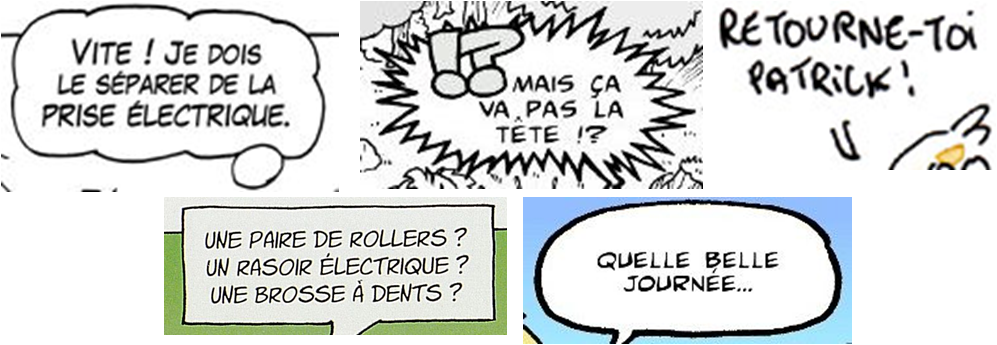
\includegraphics[width=0.65\textwidth]{balloonShape.png}
\caption[Balloon contour styles]{Balloon contour styles, from top-left to bottom-right: cloud, spiky, suggested and two smoothed contour type. Note that the two last ones are not labelled as rectangle or oval because here we annotated the type of contour and not shape (Section~\ref{sub:in:balloon_classification})}
\label{fig:gt:balloonShape}
\end{center}
\end{figure}
%%%%%%%%%%%%%%%%%%%%%%%%%%%%%%%%%%%%%%%%%%%%%%%%%%%

\paragraph{Text lines}
The text lines are associated with their transcription and the identifier of the corresponding balloon is added in \texttt{{idBalloon}} if the text line is included in a balloon.
In a second step, the function of each text line was specified through metadata \texttt{textType}. 
We identified six distinct categories of text.
The text that is used to tell the story and that can be either spoken (\texttt{speech}) or thought (\texttt{thought}) or narrated (\texttt{narrative}).
On the other hand, there are textual information that bring timely and contextual information, they are the onomatopoeia (\texttt{onomatopoeia}) and drawn text (\texttt{illustrative}) as part of the drawing such as license plate, storefront, brand.
The sixth category has been defined as notes (\texttt{note}) for embedded text in the page, such as the signature of the author, the page number, the title (every other readable text type).
%Another information have been added in 2014: the \texttt{textType} that specifies if the text is of type \{\texttt{speech, thought, onomatopoeia, narrative, illustrative, note}\}

\paragraph{Comic characters} % (fold)
\label{par:comic_characters}
The comic characters are identified by \texttt{{idCharacter}} in order to be easily referred.
Currently, it is the only metadata concerning the comic characters but it can be extended with information about character name, gender, posture, relationship etc.

% paragraph comic_characters (end)

% \paragraph{Speaking character and speech balloon} % (fold)
% \label{par:speaking_character_and_speech_balloon}
% In the second version of the ground truth, we added a new type of relation which is between regions.
%  balloons and comic characters regions that are related in the story (balloon spoken by a character).
% The information is stored in a structure called \texttt{{LinkSBSC}} that consist a pair of identifier \texttt{{idBalloon}} and \texttt{{idCharacter}}.
% paragraph speaking_character_and_speech_balloon (end)


%%%%%%%%%%%%%%%%%%%%%%%%%%%%%%%%%%%%%%%%%%%
% \begin{figure}
% \begin{center}
% \includegraphics[width=0.45\textwidth]{balloons_shape3.png}
% \caption{Different speech balloon shapes. Top-down, from left to right: cloud, peak, suggested, rectangular and oval.}
% \label{fig:balloons_shape}
% \end{center}
% \end{figure}
%%%%%%%%%%%%%%%%%%%%%%%%%%%%%%%%%%%%%%%%%%%

% section semantic_annotation (end)

\subsection{File structure} % (fold)
\label{sub:file_structure}

The ground truth file structure have been thought according to existing comics related formalism such as Comics Markup Language (ComicsML)~\cite{McIntosh2011}, Comic Book Markup Language (CBML)~\cite{Walsh2012a}, Periodical Comics\footnote{\url{http://www.w3.org/wiki/WebSchemas/PeriodicalsComics}}, A Comics Ontology~\cite{Rissen2012}, Advanced Comic Book Format (ACBF)\footnote{\url{https://launchpad.net/acbf}} and the Grand Comics Database (GCD)\footnote{\url{http://www.comics.org}}.
See the Ph.D. thesis of Gu{\'e}rin~\cite{phdthesisGuerin14} for an extended review.

As we wanted to keep the ground truth file system simple and easy to share, visual and semantic annotations about a given page are gathered in a single full-text file following the specifications of Scalable Vector Graphics (SVG). 
Besides being an open-standard developed by the World Wide Web Consortium (W3C) since 1999, the SVG format fulfils two essential needs for this database.

First, using a recent Internet browser or your favourite image viewer, it provides a simple, fast and elegant way to display the visual annotation of any desired object over a comic book page using layers.
No need to install software such as Matlab, Adobe Illustrator or equivalent open source to visualize the ground truth information.
It is an XML-based vector image format that allows to display and interact with the annotated region, stored as polygon object in the SVG file, as desired using the Cascading Style Sheets (CSS) properties (Figure~\ref{fig:gt:svgImage}). 
Each layer can be displayed or not in order to enhance the clearness of the annotations when browsing the database.

%%%%%%%%%%%%%%%%%%%%%%%%%%%%%%%%%%%%%%%%%%%%%%%%%

\begin{figure}[h!]
\begin{center}
\begin{tabular}{ccc}
a) 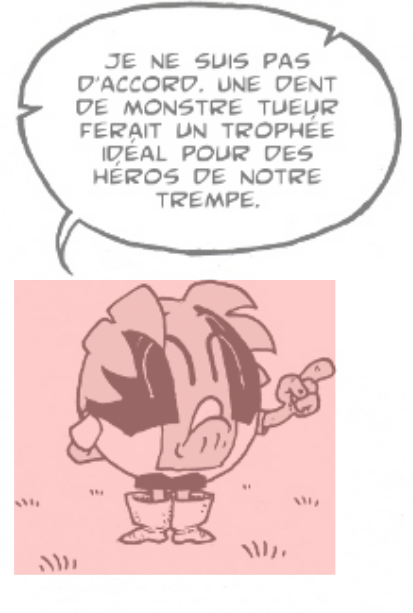
\includegraphics[width=100px]{svgPanel.png} 
& 
b) 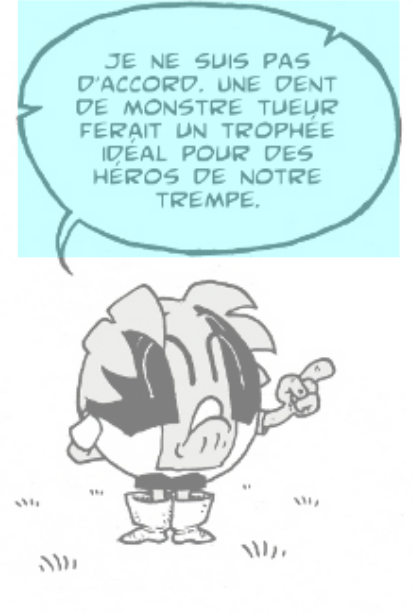
\includegraphics[width=100px]{svgBalloon.png}
&
c) 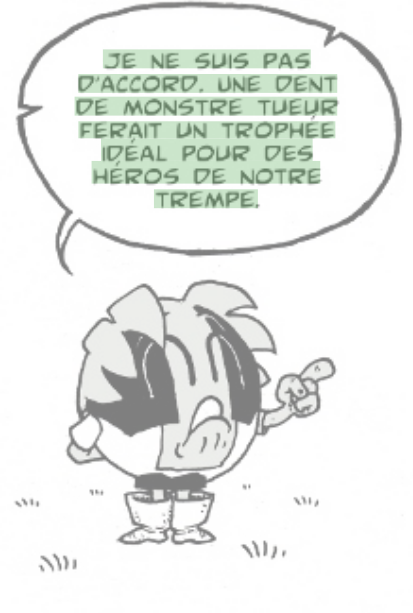
\includegraphics[width=100px]{svgTextlines.png}
\end{tabular}
\caption[Annotation rendering in a browser]{Example of rendering for each class of element. For example, red for panels (a), cyan for balloons (b) and green for text (c). The opacity is set to 50\% to allow seeing the corresponding image by transparency.} 
\label{fig:gt:svgImage}
\end{center}
\end{figure}
%%%%%%%%%%%%%%%%%%%%%%%%%%%%%%%%%%%%%%%%%%%%%%%%%%


Second, SVG being a XLM-based language, it makes the integration of semantic annotation very easy via the use of the predefined \texttt{metadata} element.

One ground truth file contains the complete description of one comics image. 
There is no hierarchical link between pages from a same comic book. 
Following the basic XML encoding information, an SVG file starts with a root \texttt{<svg>} element containing the title of the document, \texttt{<title>}, and five \texttt{<svg>} children with different class attributes.
These contain annotations collected on five types of elements which are the page, panels, balloons, text lines and comic characters.
The type of element in a tag is specified by its \texttt{class} attribute.
The first tag, \texttt{class = ``Page''} contains description on the image and has two daughters.
The first one, \texttt{image} has several attributes which specifies a link to the image file in the dataset \texttt{xlink: href} and two specifying the \texttt{width} and \texttt{height} of the image.
The second, \texttt{metadata}, contains bibliographic information about the album and page properties described in Section~\ref{sub:gt:semantic_annotation}.
%A SVG file begins with information about the XML version and encoding system and then a root \texttt{<svg>} element containing the title of the document \texttt{<title>} and four others \texttt{<svg>} elements with different class attributes. % that describe the page, the panels, the text lines and the text areas the entire set of annotations for the attached page.
%The annotations are the same for all the \texttt{<svg>} nodes, each of them describing one kind of element (e.g. panel, balloon) according to its {\tt class} attribute. 
%The first \texttt{<svg>} element, \texttt{<svg class=``Page''>}, has two children.
%The first one is \texttt{<image>} and contains a link to the corresponding image file and the size it has to be displayed.
%The next child is a \texttt{<metadata>} element containing the bibliographical information described in \ref{sub:gt:semantic_annotation}.
The four following \texttt{<svg>} siblings, \texttt{<svg class=``Panel''>}, \texttt{<svg class=``Balloon''>}, \texttt{<svg class=``Line''>} and \texttt{<svg class=``Character''>} respectively contain the annotations about panels, balloons, text lines and comic characters. 
They all contain SVG \texttt{<polygon>} elements with a list of five or more points in a \texttt{point} attribute that define the position of the bounding box corners or the pixel-level contour. %four corners position coordinates of a bounding box. 
Note that the last point is always equal the first one to ``close'' the polygon according to the SVG specifications. 
Those points are used by the viewer to draw polygons with the corresponding CSS style. 
Each \texttt{<polygon>} has a \texttt{<metadata>} child to store information on the corresponding polygon, according to the attributes list described Section~\ref{sub:gt:semantic_annotation}.
% An example of ground truth file is given Appendix~\ref{app:groundtruth}.
% présente un exemple du contenu de l'un de ces fichiers.


An example of ground truth file content is given Listing~\ref{list:svg_gt_sample}.

\begin{lstlisting}[language=XML, frame=single, caption=Example of ground truth information stored in a SVG file, captionpos=b, label=list:svg_gt_sample]
<?xml version="1.0" encoding="UTF-8" standalone="no"?>
<svg>
  <title>CYB_BUBBLEGOM_T01_005</title>
  <svg class="Page">
    <image 
      x="0" 
      y="0" 
      width="750" 
      height="1060" 
      href="CYB_BUBBLEGOM_T01_005.jpg"
    />
    <metadata 
      collectionTitle="Bubblegom_Gom"
      editorName="Studio_Cyborga" 
      doublePage="false"
      website="http://bubblegom.over-blog.com"
      albumTitle="La_Legende_des_Yaouanks"
      drawerName="Cyborg_07"
      language="french"
      resolution="300"
      ISBN="979-10-90655-01-0"
      readingDirection="leftToRight" 
      writerName="Cyborg_07"
      releaseDate="2009"
      pageNumber="5"
    />
  </svg>
  <svg class="Panel">
    <polygon points="53,95 268,95 268,292 53,292 53,95">
      <metadata 
        idPanel="P01"
        rank="1"
      />
    </polygon>
    ...
  </svg>
  <svg class="Balloon">
    <polygon points="61,103 143,103 143,172 61,172 61,103">
      <metadata
        idBalloon="B01" 
        shape="smooth"
        tailTaip="153,167"
        tailDirection="SE" 
        rank="1"
      />
    </polygon>
    ...
  </svg>
  <svg class="Line">
    <polygon points="373,121 432,121 432,132 373,132 373,121">
      <metadata 
        idLine="L01"
        idBalloon="B01"
      >
        LIKE YOU.
      </metadata>
    </polygon>
    ...
  </svg>
  <svg class="Character">
    <polygon points="84,153 261,153 261,298 84,298 84,153"/>
      <metadata idCharacter="C01"/>
    ...
  </svg>
  <svg class="LinkSBSC">
    <polygon points="34,234 56,235 79,340 79,339 34,234"/>
      <metadata 
        idLinkSBSC="LSBSC01"
        idBalloon="B01"
        idCharacter="C01"
      />
    ...
  </svg>
</svg>
\end{lstlisting}


\section{Ground truth quality assessment}
\label{sec:gt:ground_truth_quality_assessment}

When several people are involved in the creation of a graphical ground truth, it is very difficult to obtain an homogeneous segmentation.
Indeed, it could vary from one person to another because each person has a different sensitivity at reading comics and at integrating instructions.
Therefore, in addition to the package of pages he was in charge of, each participant has been asked to annotate the panels of an extra page. 
This extra page was the same for everybody and was chosen for its graphical components heterogeneity. 
It contained ten panels from which, four were full-framed, five half-framed and one was frameless.
%, see Fig. \ref{fig:test_page}. 
% This heterogeneity is somehow representative of the whole corpus.
We defined an acceptable error for the position of a corner given by several persons.
The images of dataset being of different definitions, using a percentage of the page size makes more sense than using a specific number of pixels.
%A percentage of the page width and height is more relevant.
%Let set an acceptable error of 0.5\% of the page for the position on each corner. 
We set this percentage $p$ at 0.5\% of the page height and width in $x$ and $y$. 
Given the definition of the test image of 750x1060 pixels, this makes a delta of +/- 5 pixels in $y$ axis and +/- 4 pixels in $x$ axis. 

We asked to each one of the twenty involved persons to draw the four points bounding box of the panels ignoring text area.
A mean position from the twenty different values has been calculated for each of them.
Then, the distance of each point to its mean value is computed. 
Figure~\ref{fig:gt:graphiqueStdVT} shows the amount of corners for a distance, centred on zero.


%%%%%%%%%%%%%%%%%%%%%%%%%%%%%%%%%%%%%%%%%%%%%ù
\begin{figure}[h!]
\begin{center}
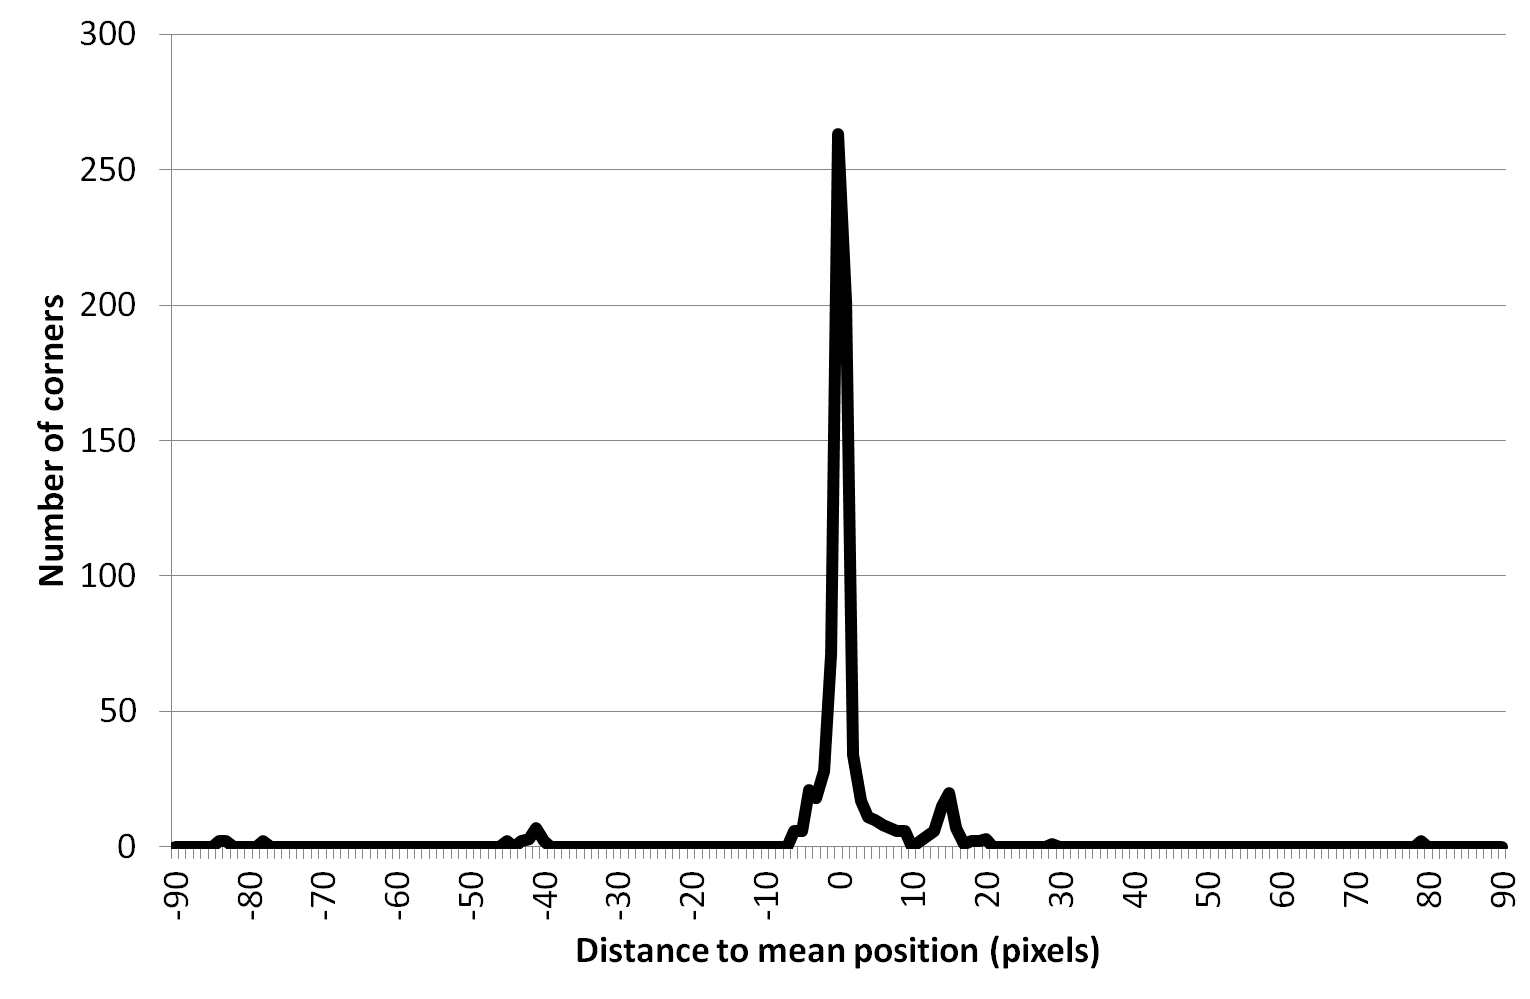
\includegraphics[width=0.7\textwidth]{stdVT.png}
\caption[Distance to the mean position]{Number of corners for a given standard deviation value. This has been calculated on $y$ axis and $x$ axis and produces similar plot.}
\label{fig:gt:graphiqueStdVT}
\end{center}
\end{figure}
%%%%%%%%%%%%%%%%%%%%%%%%%%%%%%%%%%%%%%%%%%%%%ù

Given the threshold $th=0.5$, 87.5\% of pointed corners can be considered as being homogeneous over the group of labelling people. 
%{\bf what is p?} p is the threshold
The overall mean standard deviation on this page reaches 0,15\%
 (1.13 pixels) for the width, and 0.12\% (1.28 pixels) for the height.
The two bumps, at -40 and 15, are related to the poor segmentation of 13 of the 80 panels. 
Indeed, instructions have been misunderstood by some people who included text area outside of the panels or missed some panel's parts.
Figure~\ref{fig:gt:diffVT} shows the difference between areas labelled as a panel by at least one person and areas labelled as a panel by every participants.
However, such mistakes have been manually corrected before publishing the ground truth.

%%%%%%%%%%%%%%%%%%%%%%%%%%%%%%%%%%%%%%%%%%%%%%%%%
\begin{figure}[h!]
\begin{center}
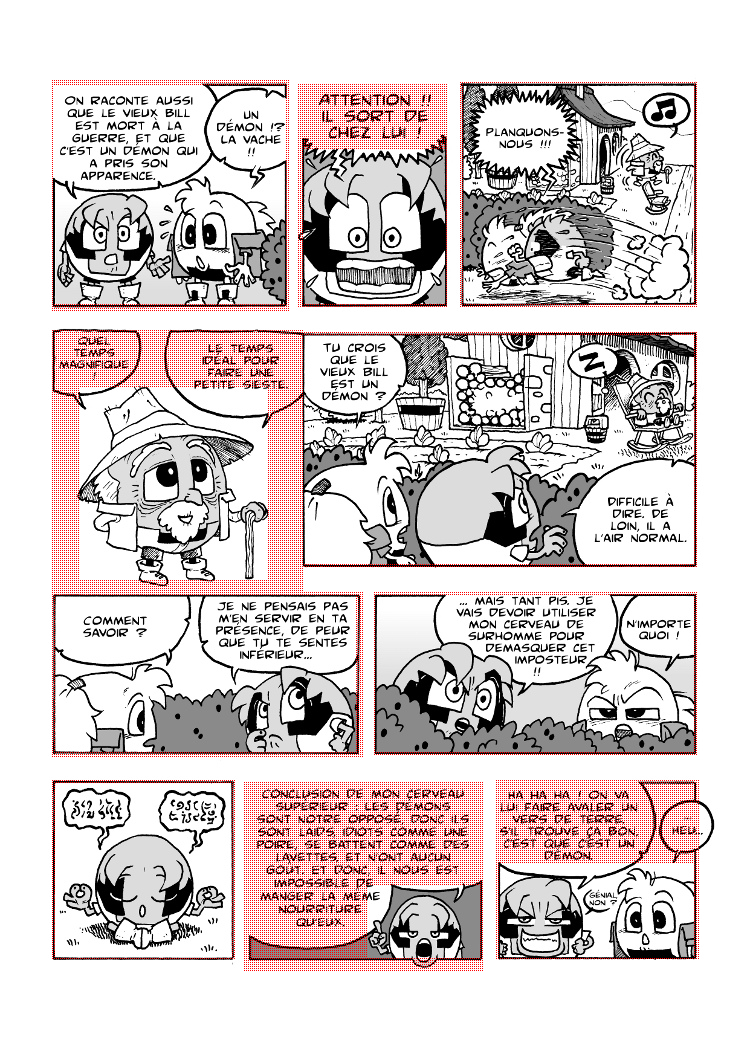
\includegraphics[width=0.7\textwidth]{segDifference.png}
\caption[Image used for ground truth quality assessment]{Image used for error measurement. Red hatched areas are the difference between areas labelled as panels by at least one person and areas labelled by everybody. Image credit:~\cite{Bubble09}.}
\label{fig:gt:diffVT}
\end{center}
\end{figure}
%%%%%%%%%%%%%%%%%%%%%%%%%%%%%%%%%%%%%%%%%%%%%%%%%

Even though the error criterion has only been estimated on panels, it is reasonable to extend it to balloons and text lines as well.
Indeed, the segmentation protocol being quite similar for all features (bounding box as close as possible to the drawing), the observed standard deviation of panel corner positions has no reason to be different from balloons and text lines.
The pixel-level balloon and the comic characters visual annotation have been carried out by a single person, the homogeneity is only subject to the regularity of the person over time and is, therefore, difficult to assess quantitatively.


\section{Terms of use} % (fold)
\label{sub:term_of_use}
We obtain the minimum rights for sharing and publishing image material from the right holders but we had to make sure the user accept it before using the data.
In collaboration with the intellectual property department of the University of La Rochelle, we established the following:

\textit{In order to use this database, you must firstly agree to the terms.
You may not use the database if you don't accept the terms.
The use of this database is limited to scientific and non-commercial purpose only, in the computer science domain.
For instance, you are allowed to split the images, through the use of segmentation algorithms.
You can also use pieces of this database to illustrate your research in publications and presentations.
Any other use case must be validated by our service.
If you do agree to be bound by all of these Terms of Use, please fill and email the request form and then use the login and password provided to download the selected version below.}

The concerned request form requires the identity, affiliation, address and intended use of the person who wishes to use data.

